\section{Differenzialrechnung}
\subsection{Vorüberlegung}
\begin{minipage}{7cm}
%%              {<x >x  <y >y
\begin{mathplot}{6}{0}{3}{0}{1}{$x$}{$y$}
\draw (0,0) -- node[above] {g} (3,1) -- (6,2);
\draw (3,1) -- (3,0);
\draw (3,0.3) node[left] {$y_1$};
\draw (2.5,1.5) node {P$_1(x_1|y_1)$};
%\draw (5,1.66) -- (5,0);
%\draw (5,0.3) node[right] {$y_2$};
\draw (4.5,2.16) node {P$_2(x_2|y_2)$};
\draw[color=red] (3,1) -- node[below] {$x_2-x_1$} (5,1);
\draw[color=orange] (5,1) -- node[right] {$y_2-y_1$} (5,1.66);
\end{mathplot}
\end{minipage}
\hfill
\begin{minipage}{8cm}
$m = \frac{y_2-y_1}{x_2-x_1} = \frac{\mathrm{\Delta}x}{\mathrm{\Delta}y}$

($\mathrm{\Delta}$-Differenz)
\end{minipage}

\subsubsection{Praktisches Beispiel}
\ZifferPunktAus
\begin{tabular}{c|c|d{1}|d{1}|d{1}|d{0}|d{2}}
	$t$ & 0 & 0,5	& 1		& 1,5	& 2		& 2,5 \\ \hline
	$s$ & 0 & 12,5	& 22,5	& 31,5	& 38	& 42,195 \\
\end{tabular}\ZifferPunktAn

\begin{minipage}{7cm}
\begin{tikzpicture}
   \FPset\fxmax{10}
    \FPset\fxmin{0}
    \FPset\fymax{5}
    \FPset\fymin{0}
%% Berechnung
    \FPadd\xmax\fxmax\gitter
    \FPadd\ymax\fymax\gitter
    \FPsub\xmin\fxmin\gitter
    \FPsub\ymin\fymin\gitter
%% Gitter
    \draw[very thin,color=gray] (\FPprint\xmin,\FPprint\ymin) grid (\FPprint\xmax,\FPprint\ymax);
%% Achsen
    \draw[->] (\xmin,0) -- (\xmax,0) node[right] {$t$};
    \draw[->] (0,\ymin) -- (0,\ymax) node[above] {$s$};
%% Zahlen
    \foreach \y in {\fymin,...,\fymax}{
      \ifthenelse{\equal{\y}{0}}{}{
        \draw (0.1,\y) -- (-0.1,\y) node[left] {\y 0};
      }
    }
    \foreach \x/\xval in {2/0.5,4/1,6/1.5,8/2,10/2.5}{
      \ifthenelse{\equal{\x}{0}}{}{
        \draw (\x,0.1) -- (\x,-0.1) node[below] {\xval};
      }
    }
    \draw[color=black, domain=\xmin:\xmax] plot[smooth=unique] file
{files/gnuplot-tables/Differenzialrechnung.PraktischesBsp.table};
    \draw[color=green] (0,0) -- (5,3.125);
    \draw[color=brown] (6,3.3805) -- (10,4.2195);
%    \draw[color=cyan] (10,0) -- (10,4.2195) node[right] {42,195};
    \draw[color=gray] (8,3.8) -- (10,3.8) -- (10,4.2195);
    \draw[color=red] (0,0) -- (10,4.2195);
%    \draw[color=blue] (0,0) -- node[above] {2,5} (10,0);
    \draw[color=black,fill] (2,1.25) circle (0.06cm);
%    \draw (1.7,1.4) node {$P_0$};
    \draw[color=black,fill] (4,2.25) circle (0.06cm);
%    \draw (3.7,2.4) node {$P$};
    \draw[color=blue,fill] (6,3.15) circle (0.06cm);
    \draw[color=blue] (6,4.5) node {P$(1{,}5|31{,}5)$};
    \draw[color=black,fill] (8,3.8) circle (0.06cm);
    \draw (10.5,3) node[right] {};
    \draw (10.5,2) node[right] {};
\end{tikzpicture}\stepcounter{mathplotcount}
\end{minipage}
\hfill
\begin{minipage}{4.7cm}
$s$ -- Weg in \si{\kilo\metre} \\
$t$ -- Zeit in \si{\hour}

%\textcolor{blue}{P$(1,5|31,5)$}
%
%\hspace{0.32cm}
%\begin{tikzpicture}
%\draw[->] (0.66,0) -- (0.66,0.3);
%\draw[->] (0,0) -- (0,0.3);
%\draw (0,-0.3) node[r] {1,5h};
%\draw (0.66,-0.3) node {31,5km};
%\end{tikzpicture}

\bigskip

$V = \frac{\SI{42}{\kilo\metre}}{\SI{2,5}{\kilo\metre}} = \SI{16,8}{\kilo\metre\per\hour}$ \\
Durchschnittsgeschwindigkeit des Läufers
\end{minipage}


\begin{multicols}{2}

\begin{tikzpicture}\draw[color=green,fill] circle (0.1cm);\end{tikzpicture}
$V_\emptyset = \frac{\SI{12,5}{\kilo\metre}}{\SI{0,5}{\kilo\metre}} = \SI{25}{\kilo\metre\per\hour}$


\begin{tikzpicture}\draw[color=brown,fill] circle (0.1cm);\end{tikzpicture}
$V_\emptyset = \frac{\SI{42}{\kilo\metre} - \SI{38}{\kilo\metre}}{\SI{2,5}{\kilo\metre} - \SI{2}{\kilo\metre}}
= \frac{\SI{4}{\kilo\metre}}{\SI{0,5}{\kilo\metre}} = \SI{8}{\kilo\metre\per\hour}$

\fbox{$V_\emptyset = \frac{S_2 - S_1}{t_2 - t_1} = \frac{\mathrm{\Delta}s}{\mathrm{\Delta}t}$}
\end{multicols}

\begin{minipage}{7cm}
\begin{mathplot}{10}{0}{5}{0}{1}{$x$}{$y$}
\draw[color=black, domain=\xmin:\xmax] plot[smooth=unique] file {files/gnuplot-tables/Differenzialrechnung.Sekante.table};
\draw[color=red] (0,1.1) -- node[sloped,above] {Tangente} (6,4.4);
\draw[color=red,<-] (2.5,2.2) -- (4.1,2.7);
\draw[color=black,fill] (2,2.2) circle (0.06cm);
\draw (2,2) node[right] {P$_0$};
\draw[color=black,fill] (4,2.9) circle (0.06cm);
\draw (4,2.7) node[right] {P};
\end{mathplot}
\end{minipage}
\hfill
\begin{minipage}{5.7cm}
Sekante $m_s$: Sekantensteigung $\rightarrow V_\emptyset$

\textcolor{red}{Tangente} $m_t$: Tangentensteigung $\rightarrow$ Augenblickliche \enquote{momentane}
Änderungsraten

$V_\emptyset = \frac{\SI{0}{\metre}}{0}$ ?
\end{minipage}

Das Grundproblem der Differenzialrechnung ist, wie man die Tangentensteigung ermitteln kann.

%\subsection{Mathematisierung des praktischen Beispiels}
\subsubsection{Mathematisierung des praktischen Beispiels}
\begin{minipage}{7cm}
\begin{mathplot}{9}{0}{5}{0}{1}{$x$}{$y$}
\draw[color=black, domain=\xmin:\xmax] plot[smooth=unique]
file {files/gnuplot-tables/Differenzialrechnung.mathPraktischesBsp.table} node[right] {$f$};
\draw[color=red] (0,1.14) -- node[sloped,above] {Tangente} (7,4.9);
\draw[color=red,<-] (2.25,2.5) -- (5.05,3.14);
\draw[color=blue] (0,1.7334) -- (7,3.366) node[right] {Sekante};
\draw[color=black,fill] (2,2.2) circle (0.06cm) node[above] {P$_0$};
\draw[color=black,fill] (5,2.9) circle (0.06cm);
\draw (4.97,3.16) node[right] {P};
\draw (2,2.2) -- node[below] {$\mathrm{\Delta}x=x-x_0$} (5,2.2) -- node[right] {$\mathrm{\Delta}y=f(x)-f(x_0)$} (5,2.9);
\end{mathplot}
\end{minipage}
\hfill
\begin{minipage}{4.7cm}
P$\big(x|f(x)\big)$

P$_0\big(x_0|f(x_0)\big)$

$m_s = \frac{f(x) - f(x_0)}{x - x_0}$

(Steigung der Sekante)
\end{minipage}

$m_s = \frac{f(x)-f(x_0)}{x-x_0}$ Differenzenquotient (Durchschnittliche Änderungsrate)

$m_t = \lim\limits_{x \rightarrow x_0}{\frac{f(x) - f(x_0)}{x - x_0}} = f'(x_0)$ 1. Ableitung

Differenzialquotient (momentane Änderungsrate)

%\section{Wann lässt sich der Differenzialquotient an einer Stelle ermitteln?}
\subsection{Wann lässt sich der Differenzialquotient an einer Stelle ermitteln?}
%\subsection{Stetigkeit}
\subsubsection{Stetigkeit}
\begin{mathplot}{2}{-3}{4}{-1}{1}{$x$}{$y$}
\draw[color=black, domain=\xmin:\xmax] plot[smooth=unique] file
{files/gnuplot-tables/Differenzialrechnung.bspStetig1.table};
\draw (-3,0.2) -- (1,3.8);
\draw (-1,0) -- (-1,0.2) node[above] {$x_0$};
%\draw[->] (-1.5,2.5) node[above] {$x_0$} -- (-1.05,2.05);
\end{mathplot}\hspace{0.5cm}
\begin{mathplot}{2}{-3}{4}{-1}{1}{$x$}{$y$}
\draw[color=black, domain=\xmin:\xmax] plot[smooth=unique] file
{files/gnuplot-tables/Differenzialrechnung.bspStetig2-1.table};
\draw[color=black, domain=\xmin:\xmax] plot[smooth=unique] file
{files/gnuplot-tables/Differenzialrechnung.bspStetig2-2.table};
\draw (-1,0) -- (-1,0.2) node[above] {$x_0$};
%\draw[->] (-1.5,2.5) node[above] {$x_0$} -- (-1.05,2.05);
\draw (-1.05,1.95) rectangle (-0.95,2.05);
\end{mathplot}

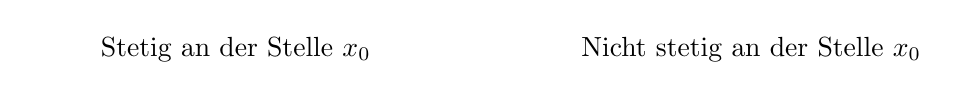
\begin{tikzpicture}
\draw (0.8,0) node[right] {Stetig an der Stelle $x_0$};% (0.6,0.3) -- (1.5,1);
\draw (6.9,0) node[right] {Nicht stetig an der Stelle $x_0$};% (8.2,0.6) -- (8.65,1);
\draw (0,0);
\end{tikzpicture}


\begin{mathplot}{2}{0}{4}{-2}{1}{$x$}{$y$}
\draw[color=black, domain=\xmin:\xmax] plot[smooth=unique] file
{files/gnuplot-tables/Differenzialrechnung.bspStetig3-1.table};
\draw[color=black, domain=\xmin:\xmax] plot[smooth=unique] file
{files/gnuplot-tables/Differenzialrechnung.bspStetig3-2.table};
\draw[->] (0.5,1.5) node[above] {$x_0$} -- (0.95,1.05);
\draw (0.95,0.95) rectangle (1.05,1.05);
\end{mathplot}
\begin{tikzpicture}
\draw[thick,<-] (0,3) -- (0.7,3) node[right] {Nicht stetig an der stelle $x_0$};
\draw[thick,->] (6,3) --(6.7,3);
%\draw[thick,<-] (0,3) -- (0.7,3) node[right] {Nicht stetig an der stelle $x_0$} (6.8,3) --(6.5,3);
\draw (0,0);
\end{tikzpicture}
\begin{mathplot}{2}{0}{5}{-1}{1}{$x$}{$y$}  % function{(x-1)**(-2)};
\draw[scale=1,color=black, domain=\fxmin:\fxmax] plot file {files/gnuplot-tables/Differenzialrechnung.bspStetig4-1.table};
\draw[scale=1,color=black, domain=\fxmin:\fxmax] plot file {files/gnuplot-tables/Differenzialrechnung.bspStetig4-2.table};
\draw (1,0) -- (1,0.2) node[above] {$x_0$};
%\draw[->] (1.1,0.5) node[left] {$x_0$} -- (1.4,0.5);
%\draw (1.45,0.45) rectangle (1.55,0.55);
\end{mathplot}

Der Differenzialquotient einer Funktion an einer Stelle $x_0$ lässt sich nur bilden, wenn die Funktion an
der Stelle $x_0$ stetig ist.

%\subsection{Differenzierbarkeit}
\subsubsection{Differenzierbarkeit}
\begin{mathplot}{3}{-3}{5}{-1}{1}{$x$}{$y$}
%\draw[samples=700, color=black, domain=-2.235:2.235] plot[id=ZeichnerischeL] function{x**2} node[above] {$x^2$};
\draw[color=black, domain=\xmin:\xmax] plot file {files/gnuplot-tables/Differenzialrechnung.ZeichnerischeL.table}
node[above] {$x^2$};
%\draw[color=black, domain=\xmin:\xmax] plot[smooth=unique] file {Differenzialrechnung.bspStetig3-2.table};
\draw[->] (0.5,1.5) node[above] {$x_0$} -- (0.95,1.05);
\draw[color=red] (0,-1) -- (3,5);
\draw (0,-1.5) node {Differenzierbar an der Stelle $x_0$};
\end{mathplot}
\begin{mathplot}{3}{-3}{5}{-1}{1}{$x$}{$y$}
\draw[color=black, domain=\xmin:\xmax] plot[smooth=unique] file
{files/gnuplot-tables/Differenzialrechnung.differenzierbar2-1.table};
\draw[color=black, domain=\xmin:\xmax] plot[smooth=unique] file
{files/gnuplot-tables/Differenzialrechnung.differenzierbar2-2.table};
\draw[->] (1.2,2.2) node[above] {$x_0$ -- Knick} -- (1,1.1);
\draw (0,-1.5) node {Nicht differenzierbar an der Stelle $x_0$};
\end{mathplot}

Der Differenzialquotient einer Funktion an einer Stelle $x_0$ lässt sich nur bilden, wenn die Funktion an
der Stelle $x_0$ differenzierbar ist.

Differenzierbarkeit ist eine stärkere Eigenschaft als Stetigkeit, dass heißt die Differenzierbarkeit schließt die
Stetigkeit mit ein. Die Stetigkeit zieht aber nicht automatisch die Differenzierbarkeit nach sich.

%\section{Ermittlung des Anstiegs einer Tangente an einer Stelle $x_0$ einer Funktion}
\subsection{Ermittlung des Anstiegs einer Tangente an einer Stelle $x_0$ einer Funktion}
$f(x) = x^2$

$x_{01} = -1$; $x_{02} = 0$; $x_{03} = 1;$

%\subsection{Zeichnerische Lösung}
\subsubsection{Zeichnerische Lösung}
%%              {<x >x  <y >y
\begin{mathplot}{3}{-3}{5}{-1}{1}{$x$}{$y$}
%\draw[samples=700, color=black, domain=-2.235:2.235] plot[id=ZeichnerischeL] function{x**2} node[above] {$x^2$};
\draw[color=black, domain=-2.18:2.18] plot file {files/gnuplot-tables/Differenzialrechnung.ZeichnerischeL.table}
node[above] {$x^2$};
\draw[color=red] (0,-1) -- (-3,5);
\draw[color=green] (\fxmin,0) -- (\fxmax,0);
\draw[color=blue] (0,-1) -- (3,5);
\draw[color=red] (4,3) node[right] {$m_1=-2$};
\draw[color=green] (4,2) node[right] {$m_2=0$};
\draw[color=blue] (4,1) node[right] {$m_3=2$};
\end{mathplot}

%\subsection{rechnerische Lösung}
\subsubsection{rechnerische Lösung}
\begin{list}{}{}
    \item[$x_{01}$:] $\lim\limits_{x \rightarrow x_0}{\frac{f(x)-f(x_0)}{x-x_0}} = \lim\limits_{x \rightarrow
-1}{\frac{x^2-(-1)^2}{x-(-1)}} = \lim\limits_{x \rightarrow
-1}{\frac{x^2-1}{x+1}} = \lim\limits_{x \rightarrow
-1}{\frac{\cancel{(x+1)}(x-1)}{\cancel{x+1}}} = \lim\limits_{x \rightarrow
-1}{(x-1)} = -2 = m_1 = f'(-1)$
    \item[$x_{02}$:] $\lim\limits_{x \rightarrow x_0}{\frac{f(x)-f(x_0)}{x-x_0}} = \lim\limits_{x \rightarrow
0}{\frac{x^2-0^2}{x-1}} = \lim\limits_{x \rightarrow
0}{\frac{x^2}{x}} = \lim\limits_{x \rightarrow 0}{x} = 0 = m_2 = f'(0)$
    \item[$x_{03}$:] $\lim\limits_{x \rightarrow x_0}{\frac{f(x)-f(x_0)}{x-x_0}} = \lim\limits_{x \rightarrow
1}{\frac{x^2-1^2}{x-1}} = \lim\limits_{x \rightarrow 1}{\frac{(x+1)\cancel{(x-1)}}{\cancel{x-1}}} =
\lim\limits_{x \rightarrow 1}{(x+1)} = 2 = m_3 = f'(1)$
\end{list}

%\section{Formel zur Tangentensteigungsberechnug}
\subsection{Formel zur Tangentensteigungsberechnug}
$\lim\limits_{x \rightarrow x_0}{\frac{f(x)-f(x_0)}{x-x_0}} =
\lim\limits_{x \rightarrow x_0}{\frac{x^2-x_0^2}{x-x_0}} =
\lim\limits_{x \rightarrow x_0}{\frac{\cancel{(x-x_0)}(x+x_0)}{\cancel{x-x_0}}} =
\lim\limits_{x \rightarrow x_0}{(x+x_0)} = 2x_0 = m_t = f'(x_0)$

\vspace{0.2cm}
\fbox{$f(x) = x^2 \rightarrow f'(x) = 2x $}

%\section{Ableitungen einiger wichtiger Grundfunktionen}
\subsection{Ableitungen einiger wichtiger Grundfunktionen}
\begin{enumerate}
    \item $f(x)=c$\\
    $f(x)=3$; $g(x)=-2$\\
    %%              {<x >x  <y >y
    \begin{mathplot}{3}{-3}{3}{-2}{1}{$x$}{$y$}
      \draw[color=green] (\fxmin,3) -- (\fxmax,3) node[right] {$f(x) = 3$};
      \draw[color=blue] (\fxmin,-2) -- (\fxmax,-2) node[right] {$g(x) = -2$};
    \end{mathplot}\\
    %\begin{multicols}{2}
    $f(x) = 3 \rightarrow f'(x) = 0$\\
    $g(x) = -2 \rightarrow g'(x) = 0$

    \vspace{0.1cm}
    \fbox{$f(x) = c \rightarrow f'(x) = 0$}\\
    Die Ableitung eines Summanden ist immer Null.
    $\lim\limits_{x \rightarrow x_0}{\frac{c-c}{x-x_0}} =
    \lim\limits_{x \rightarrow x_0}{\frac{0}{x-x_0}} =
    \lim\limits_{x \rightarrow x_0}{0} = 0$
    %\end{multicols}
    \item %\begin{multicols}{2}
    $f(x) = x$\\
    $\lim\limits_{x \rightarrow x_0}{\frac{(x-x_0)^1}{(x-x_0)^1}} =
    \lim\limits_{x \rightarrow x_0}{1} = 1$

    \vspace{0.1cm}
    \fbox{$f(x) = x \rightarrow f'(x) = 1$}\\
    Die Ableitung von $x$ ist Eins.
    %\end{multicols}
    \item %\begin{multicols}{2}
    $f(x) = mx$\\
    $\lim\limits_{x \rightarrow x_0}{\frac{mx-mx_0}{x-x_0}} =
    \lim\limits_{x \rightarrow x_0}{\frac{m\cancel{(x-x_0)}}{\cancel{x-x_0}}} =
    \lim\limits_{x \rightarrow x_0}{m} = m$

    \vspace{0.1cm}
    \fbox{$f(x) = mx \rightarrow f'(x) = m$}\\
    Die Ableitung eines Vielfachen von $x$ ist der Faktor $m$.
    %\end{multicols}
    \item \begin{multicols}{2}
        $f(x) = x^{n}$ (Potenzregel)\\
        $f(x) = x \rightarrow f'(x) = 1x^{0}$\\
        $f(x) = x^{2} \rightarrow f'(x) = 2x^{1}$\\
        $f(x) = x^{3} \rightarrow f'(x) = 3x^{2}$\\
        $f(x) = x^{4} \rightarrow f'(x) = 4x^{3}$\\
    \fbox{$f(x) = x^{n} \rightarrow f'(x) = nx^{n-1}$}\\
    Eine Potenz wird folgendermaßen abgeleitet: 1.~Der Exponent wird Faktor. \\
    2.~Der Exponent wird danach um Eins erniedrigt (dekrementiert).\\
    Die Potenzregel gilt auch, wenn der Exponent keine natürliche Zahl ist.
    \end{multicols}
\end{enumerate}

%\newpage
%\subsection{Musteraufgaben}
\subsubsection{Musteraufgaben}
\begin{multicols}{2}
\begin{enumerate}
    \item $f(x) = x^7 \rightarrow f'(x) =7x^6$
    \item $f(x) = x^{17} \rightarrow f'(x) = 17x^{16}$
    \item $f(x) = x^{-2} \rightarrow f'(x) = -2x^{-3}$
    \item $f(x) = x^{\frac{1}{3}} \rightarrow f'(x) = \frac{1}{3}x^{-\frac{2}{3}}$
    \item $f(x) = x^b \rightarrow f'(x) = bx^{b-1}$
    \item $f(x) = x^{-b} \rightarrow f'(x) = -bx^{-b-1}$
    \item $f(x) = x^{a+1} \rightarrow f'(x) = (a+1)x^a$
    \item $f(x) = \frac{1}{x}$\\
    $a^{-k} = \frac{1}{a^k}\quad (a \neq 0)$\\
    $f'(x) = -1x^{-2} = -\frac{1}{x^2}$
    \item $f(x) = \frac{1}{x^3} = x^{-3} \rightarrow f'(x) = -3x^{-4} = -\frac{3}{x^4}$
    \item $f(x) = \sqrt{x} = x^{\frac{1}{2}}\\
    a^{\frac{m}{n}} = \sqrt[n]{a^m}$\\
    $f'(x) = \frac{1}{2}x^{-1/2} = \frac{1}{2x^{1/2}} = \frac{1}{2\sqrt{x}}$
\end{enumerate}
\end{multicols}

%\section{Faktorregel}
\subsection{Faktorregel}
$f(x) = a\cdot u(x)\quad$ \zB $f(x)=3x^7$\\
$\lim\limits_{x \rightarrow x_0}{\frac{f(x)-f(x_0)}{x-x_0}} =
\lim\limits_{x \rightarrow x_0}{\frac{a\cdot u(x)-a\cdot u(x_0)}{x-x_0}} =
\lim\limits_{x \rightarrow x_0}{[\frac{u(x)-u(x_0)}{1(x-x_0)}\cdot\frac{a}{1}]} =
\lim\limits_{x \rightarrow x_0}{\frac{a}{1}}\cdot\lim\limits_{x \rightarrow x_0}{\frac{u(x)-u(x_0)}{1(x-x_0)}} =
a\cdot u'(x_0)$

\vspace{0.2cm}
\fbox{$f(x) = a \cdot u(x) \rightarrow f'(x) = a \cdot u'(x)$}\\
Ein konstanter Faktor wird bei der Bildung der Ableitung beibehalten.\\
Unterschied: Ein Summand wird dagegen Null.

\begin{multicols}{2}
$f(x) = 3\cdot x^7$\\
$f'(x) = 3\cdot 7x^6 = 21\cdot x^6$\\
$f(x) = \frac{1}{4}\cdot x^3$\\
$f'(x) = \frac{1}{4}\cdot 3x^2 = \frac{1}{4}x^2$
\end{multicols}


%\section{Summenregel}
\subsection{Summenregel}
$f(x) = u(x)+v(x)\quad$ \zB $f(x)=x^3+x^2$\\
$\lim\limits_{x \rightarrow x_0}{\frac{f(x)-f(x_0)}{x-x_0}} =
\lim\limits_{x \rightarrow x_0}{\frac{u(x)+v(x)-[u(x_0)+v(x_0)]}{x-x_0}} =
\lim\limits_{x \rightarrow x_0}{\frac{u(x)+v(x)-u(x_0)-v(x_0)}{x-x_0}}$=\\
$\lim\limits_{x \rightarrow x_0}{\frac{u(x)-u(x_0)+v(x)-v(x_0)}{x-x_0}} =
\lim\limits_{x \rightarrow x_0}{\frac{u(x)-u(x_0)}{x-x_0}}+\lim\limits_{x \rightarrow x_0}{\frac{v(x)-v(x_0)}{x-x_0}} =
u'(x_0) + v'(x_0)$

\vspace{0.2cm}
\fbox{$f(x) = u(x) \pm v(x) \rightarrow f'(x) = u'(x) \pm v'(x)$}

Eine Summe wird Summandenweise abgeleitet.\\
Zwei Hinweise: 1.~Die Summenregel gilt auch, wenn mehr als zwei Summanden beteiligt sind.
2.~Die Summenregel gilt auch, wenn die Teilfunktionen durch Subtraktion verknüpft sind.

%\section{Erste- zweite- und weitere Ableitungen von Funktionen}
\subsection{Erste- zweite- und weitere Ableitungen von Funktionen}
\begin{multicols}{3}
$f(x) = x^3 + 2x^2 - 5$\\
$f'(x) = 3x^2 + 4x$\\
$f''(x) = 6x + 4$\\
$f'''(x) = 6$\\
$f^{(4)}(x) = 0$\\
$f^{(5)}(x) = 0$
\end{multicols}

Wird eine Funktion abgeleitet, erhält man die 1.~Ableitung.
Diese 1.~Ableitung (Ableitungsfunktion) lässt sich erneut ableiten, dabei erhält man die 2.~Ableitung.
Da dieses Vorgehen aber auch für die 2.~Funktion angewendet werden kann, kann man zur 3.~Ableitung gelangen
und so weiter.

%\subsection{Musteraufgaben}
\subsubsection{Musteraufgaben}
\begin{multicols}{2}
\begin{enumerate}
    \item $f(x) = \frac{1}{4}x^4-\frac{1}{2}x^3+x$\\
    $f'(x) = x^3-\frac{3}{2}x^2+1$\\
    $f''(x) = 3x^2-3x$\\
    $f'''(x) = 6x-3$
    \item $f(x) = 2(\frac{1}{2}x^4+3x^3) = x^4+6x^3$\\
    $f'(x) = 4x^3+18x^2$\\
    $f''(x) = 12x^2+36x $\\
    $f'''(x) = 24x+36 $
    \item $f(x) = (1-\frac{1}{2}x)(x^2+1)$\\
    $= x2+1-\frac{1}{2}x^3-\frac{1}{2}x$\\
    $= -\frac{1}{2}x^3+x^2-\frac{1}{2}x+1$\\
    $f'(x) = -\frac{3}{2}x^2+2x-\frac{1}{2}$\\
    $f''(x) = -3x+2$\\
    $f'''(x) = -3$
    \item $f(x) = x^5\sqrt{2}-\frac{1}{2}x^2+2\sqrt{3}$\\
    $f'(x) = 5x^4\sqrt{2}-x$\\
    $f''(x) = 20x^3\sqrt{2}-1$\\
    $f'''(x) = 60x^2\sqrt{2}$
    \item $f(x) = \frac{3x^3-6x^2+5}{2} = \frac{3}{2}x^3-3x^2+\frac{5}{2}$\\
    $f'(x) = \frac{9}{2}x^2-6x$\\
    $f''(x) = 9x-6$\\
    $f'''(x) = 9$
    \item $f(x) = ax^3-b$\\
    $f'(x) = 3ax^2$\\
    $f''(x) = 6ax$\\
    $f'''(x) = 6a$
    \item $f(x) = k^3x+k^2x^3$\\
    $f'(x) = k^3+3k^2+x^2$\\
    $f''(x) = 6k^2x$\\
    $f'''(x) = 6k^2$
    \item $f(x) = (a^3+x^3)^2 = a^6+2a^3+x^3+x^6$\\
    $f'(x) = 6a^3x^2+6x^5$\\
    $f''(x) = 12a^3x+30x$\\
    $f'''(x) = 36a^2+30$
\end{enumerate}
\end{multicols}

Haben Funktionen Formen, die nicht unserem Regelwerk entsprechen,
muss man durch geeignete Umwandlungen (\zB Zerlegungen, Klammerauflösungen, binomische Formeln)
in eine regelgerechte Form überführen.\\
Potenzen, die im Nenner einer Funktion stehen beziehungsweise Wurzeln,
können durch die Potenzgesetze ebenso in eine regelgerechte Form überführt werden.

$f(x) = \frac{1}{x^n} = \textcolor{blue}{x^{-n}}$ \hspace{0.7cm}(\textcolor{blue}{regelgerechte Form})\\
$f(x) = \sqrt[n]{x^1} = \textcolor{blue}{x^{1/n}}$

\newpage
%\subsection{Musteraufgaben mit variierender Funktionsvariable}
\subsubsection{Musteraufgaben mit variierender Funktionsvariable}
\begin{multicols}{2}
\begin{enumerate}
    \item $f(\textcolor{red}{x}) = a\textcolor{red}{x}^3-b$\\
    $f'(\textcolor{red}{x}) = 3a\textcolor{red}{x}^2$\\
    $f''(\textcolor{red}{x}) = 6a\textcolor{red}{x}$\\
    $f'''(\textcolor{red}{x}) = 6a$
    \item $f(\textcolor{red}{x}) = k^3\textcolor{red}{x}+k^2\textcolor{red}{x}^3$\\
    $f'(\textcolor{red}{x}) = k^3+3k^2\textcolor{red}{x}^2$\\
    $f''(\textcolor{red}{x}) = 6k^2\textcolor{red}{x}$\\
    $f'''(\textcolor{red}{x}) = 6k^2$
    \item $A(\textcolor{red}{x}) = \big(a^3+\textcolor{red}{x}^3\big)^2 =
    a^6+2a^3\textcolor{red}{x}^3+\textcolor{red}{x}^6$\\
    $A'(\textcolor{red}{x}) = 6a^3\textcolor{red}{x}^2+6\textcolor{red}{x}^5$\\
    $A''(\textcolor{red}{x}) = 12a^3\textcolor{red}{x}+30\textcolor{red}{x}^4$\\
    $A'''(\textcolor{red}{x}) = 12a^3+120\textcolor{red}{x}^3$
    \item $h(\textcolor{red}{t}) = 3\textcolor{red}{t}^2-\textcolor{red}{t}^3$\\
    $h'(\textcolor{red}{t}) = 6\textcolor{red}{t}-3\textcolor{red}{t}^2$\\
    $h''(\textcolor{red}{t}) = 6-6\textcolor{red}{t}$\\
    $h'''(\textcolor{red}{t}) = -6$
    \item $h(\textcolor{red}{a}) = \textcolor{red}{a}b^2+\textcolor{red}{a}^2b+c$\\
    $h'(\textcolor{red}{a}) = b^2+2\textcolor{red}{a}b$\\
    $h''(\textcolor{red}{a}) = 2b$\\
    $h'''(\textcolor{red}{a}) = 0$
\end{enumerate}
\end{multicols}
